%======================================================
% This file is part of
% "AMCOS_booklet"
% Version 1.1 (04/07/2019)
% A LaTeX template for conference books of abstracts
%
% This template is available at:
% https://github.com/maximelucas/AMCOS_booklet
%
% License: GNU General Public License v3.0
%
% Authors:
% Maxime Lucas (ml.maximelucas@gmail.com)
% Pau Clusella
%=======================================================

\documentclass[openany, parskip=full, 12pt, a4]{scrbook}

%======================================================
% This file is part of
% "AMCOS_booklet"
% Version 1.1 (04/07/2019)
% A LaTeX template for conference books of abstracts
%
% This template is available at:
% https://github.com/maximelucas/AMCOS_booklet
%
% License: GNU General Public License v3.0
%
% Authors:
% Maxime Lucas (ml.maximelucas@gmail.com)
% Pau Clusella
%=======================================================

\usepackage[utf8]{inputenc}
\usepackage[T1]{fontenc}

%---------------------------------------------------------
% PACKAGES
%---------------------------------------------------------

% TYPOGRAPHY
\usepackage{xspace}
\usepackage{microtype}
\usepackage{cmbright} % different fonts

% VARIA
\usepackage{color}
\usepackage[table]{xcolor} % loads also »colortbl« %load before tikz if options
\usepackage{tabularx}      % For tables with specified width
\usepackage{scrhack} % fix koma script warning about addtolist
\usepackage{blindtext}
\usepackage{pdfpages} % for cover 

\usepackage{ifthen} % to have online and printed versionw

% GRAPHICS & FIGURES & TABLES
\usepackage{graphicx}
\usepackage{float}
\usepackage{multicol} % for timetable
\usepackage{longtable} % for list of participants over more than 1 page
%\usepackage{wrapfig}
%\usepackage{tikz}
%\tikzset{ar/.style={>=latex, ->}}
%\renewcommand{\arraystretch}{1.2}
%\usepackage[multidot]{grffile}
% \usepackage{booktabs}

% WANTS TO BE LAST
\usepackage[english]{babel}

\usepackage[hidelinks]{hyperref}
\hypersetup{pdfpagelayout=TwoPageRight}
% \usepackage[ocgcolorlinks]{hyperref}
% \hypersetup{colorlinks, linkcolor={wolf}, linktocpage=true, citecolor ={tpred}, urlcolor={black}}


%-------------------------------------------------------------
% SETTINGS
%-------------------------------------------------------------
\pagestyle{plain}

\setcounter{secnumdepth}{-2} % remove numbering at any level both for the heading and the toc
%https://tex.stackexchange.com/questions/30122/generate-table-of-contents-when-section-sections-without-numbering-has-been

%-------------------------------------------------------------
% USEFUL DEFINTIONS
%-------------------------------------------------------------

% VARIA 
\newcommand\tab[1][1cm]{\hspace*{#1}}

%======================================================
% This file is part of
% "AMCOS_booklet"
% Version 1.1 (04/07/2019)
% A LaTeX template for conference books of abstracts
%
% This template is available at:
% https://github.com/maximelucas/AMCOS_booklet
%
% License: GNU General Public License v3.0
%
% Authors:
% Maxime Lucas (ml.maximelucas@gmail.com)
% Pau Clusella
%=======================================================

%
% COLORS
%

\definecolor{myorange}{RGB}{255,117,40}
\definecolor{mygray}{RGB}{164, 168, 172}
\definecolor{mywhite}{RGB}{235, 238, 231}
\definecolor{myblue}{RGB}{52, 115, 116}
\definecolor{etd2024}{RGB}{60, 120, 216}

\newcommand{\primarycolor}{etd2024}
\newcommand{\secondarycolor}{mywhite}
\newcommand{\ternarycolor}{mywhite}

%
% BOOKLET VERSIONS
%

% If compilation is done with 'compile.sh', both versions (online and printed) are automatically compiled
% If compilation is done from editor, choose which version to compile below
\makeatletter
\@ifundefined{ifOnline}{% % check if already defined from the command line, if not define \ifOnline
	\expandafter\newif\csname ifOnline\endcsname
	\Onlinefalse %set to \Onlinefalse/\Onlinetrue for printed/online version
}{}
\makeatother

% define \type to input the right version of the abstracts
\ifOnline
\newcommand{\type}{o}
\else
\newcommand{\type}{p}
\fi % end if

%
% ABSTRACT ENVIRONMENTS
%

%----------------------------------------
% online abstract environment
%----------------------------------------
\newenvironment{abstract_online}[4] %{title}{author}{affiliation}{type}
{\filbreak %avoid page break
	
	{\large \bfseries #1}
	
	{\bfseries \itshape #2} \hfill {#3}
	
	\textcolor{mygray}{#4}
	
}
{}

%----------------------------------------
% talk abstract environment (printed)
%----------------------------------------
\newenvironment{abstract}[4] %{title}{author}{affiliation}
{\filbreak %avoid page break
	
	{\large \bfseries #1}
	
	{\bfseries \itshape #2,} \textcolor{mygray}{#3} \hfill {#4}
	
	
}
{}

%----------------------------------------
% poster abstract environment (printed)
%----------------------------------------
\newcommand{\poster}[3] %{title}{author}{affiliation}
{\filbreak %avoid page break
	
	{\bfseries \large #1} \\	
	\tab #2, \textit{#3}
	
}
{}

%----------------------------------------
% tags for talk type (colored circle in abstracts)
%----------------------------------------

\newcommand{\KLtag}{\tikz[baseline={([yshift=-.8ex]current bounding box.center)}]  \node[circle, inner sep=2pt, minimum size=0.5em, color=black, fill=\KLcolor]{\small \bfseries KL};} %colored circle with tag

\newcommand{\IStag}{\tikz[baseline={([yshift=-.8ex]current bounding box.center)}]  \node[circle, inner sep=2pt, minimum size=0.5em, color=black, fill=\IScolor]{\small \bfseries IS};} %colored circle with tag

\newcommand{\CTtag}{\tikz[baseline={([yshift=-.8ex]current bounding box.center)}]  \node[circle, inner sep=2pt, minimum size=0.5em, color=black, fill=\CTcolor]{\small \bfseries CT};} %colored circle with tag

\newcommand{\ITtag}{\tikz[baseline={([yshift=-.8ex]current bounding box.center)}]  \node[circle, inner sep=2pt, minimum size=0.5em, color=black, fill=\ITcolor]{\small \bfseries IT};} %colored circle with tag

%
% PAGE LAYOUT DEFINITIONS
%
\usepackage{etoolbox}

%------------------------------------------------------
% page style: vertical line on the side of each page
%------------------------------------------------------
\usepackage[scale=1,angle=0,opacity=1]{background}
\backgroundsetup{contents={}}

\AddEverypageHook{%
\ifthenelse{%
	\isodd{\thepage} \AND  \thepage>1 % if odd page but not front page
	}{%
	\backgroundsetup{
		color=\secondarycolor,
		position=current page.south east,%
		nodeanchor=south east,
		contents={\rule{10pt}{0.66\paperheight}}
		}
	}{%
	% nothing
	}
%
\ifthenelse{% 
	\NOT \isodd{\thepage} \AND \NOT \thepage=44% if even page
	}{%
	\backgroundsetup{
		color=\secondarycolor,
		position=current page.south west,%
		nodeanchor=south west,
		contents={\rule{10pt}{0.66\paperheight}}
		}
	}{%
	% nothing
	}
\BgMaterial}


%---------------------------------------------------
% chapter heading style
%---------------------------------------------------

\newdimen\mybarpadding
\mybarpadding=1.5em\relax %padding between gcolored bar and chapter name

\RedeclareSectionCommand[%
    ,afterskip=4em plus 1pt minus 1pt%
    ,beforeskip=-1pt%1.2em plus 1pt minus 1pt%
    ,level=0%
    ,toclevel=0%
]{chapter}%

\setkomafont{chapter}{\normalfont\normalsize\bfseries\Huge} % koma-script-specific command

\newcommand*{\mynumberedtest}[1]{% to test whether there is a number
  \if\relax\detokenize{#1}\relax%
  \else%
    #1%
    
  \fi}

%-------------------------------------------------chapter style definition

\renewcommand{\chapterlinesformat}[3]{%
  \ifthispageodd{%
    \hfill%
    \raisebox{-0.2em}{%
      \makebox[0pt][r]{\textcolor{\primarycolor}{\rule{\paperwidth}{1em}}}%
    }%
    \hspace{\mybarpadding}%
% 	\mynumberedtest{#2}
	\mbox{#3}%
  }{%
%    \hbox{%
%       \mynumberedtest{#2}
      \mbox{#3}%
      \hspace{\mybarpadding}%
      \raisebox{-0.2em}{%
        \makebox[0pt][l]{\textcolor{\primarycolor}{\rule{\paperwidth}{1em}}}%
      }%
%    }%
  }%
}
\makeatother
%---------------------------------------------------------

% TIMETABLE COLORS AND STYLES

% text and backgroud colors
\newcommand{\tbg}{gray} % background
\newcommand{\tfg}{white}
\newcommand{\tbc}{gray!25}

% talk types colors
\newcommand{\IScolor}{myblue!65} % invited speaker
\newcommand{\CTcolor}{white} % contributed talk
\newcommand{\KLcolor}{myorange!45} % keynote lecture
\newcommand{\ITcolor}{yellow!25} %

% row types
\newcommand{\tablebreak}[2]{% {time span}{break name}
	\rowcolor{\tbc} #1 &  \multicolumn{4}{c|}{\bfseries #2} \\ \hline }
\newcommand{\eventtype}[2]{% {time span}{event name}
	#1& \multicolumn{4}{c|}{\cellcolor{\tbg}\color{\tfg}\bfseries #2} \\ \hline }

% column spacing and position
\newcolumntype{L}[1]{%
	>{\raggedright\let\newline\\\arraybackslash\hspace{0pt}}m{#1}}
\newcolumntype{C}[1]{%
	>{\centering\let\newline\\\arraybackslash\hspace{0pt}}m{#1}}
\newcolumntype{R}[1]{%
	>{\raggedleft\let\newline\\\arraybackslash\hspace{0pt}}m{#1}}

%\newcommand{\mytable}{|C{0.15\linewidth}| C{0.05\linewidth}|  C{0.25\linewidth} C{0.1\linewidth} C{0.5\linewidth}|}

\newcommand{\IS}[5]{% {time span}{name}{University}{City, Country}{title}
	#1 &\cellcolor{\IScolor}IS&{\bfseries#2}\newline #4&&#5 \\ \hline}
\newcommand{\CT}[5]{%
	#1 &\cellcolor{\CTcolor}CT&{\bfseries#2}\newline #4&&#5 \\ \hline}
\newcommand{\KL}[5]{%
	#1 &\cellcolor{\KLcolor}KL&{\bfseries#2}\newline #4&&#5 \\ \hline}
\newcommand{\IT}[5]{%
	#1 &\cellcolor{\ITcolor}IT&{\bfseries#2}\newline #4&&#5 \\ \hline}
\newcommand{\tutorial}[5]{%
	#1 && {\bfseries#2}\newline #4 &&#5 \\ \hline}

	
\begin{document}

% COVER PAGE
%--------------------------------------------------------------------
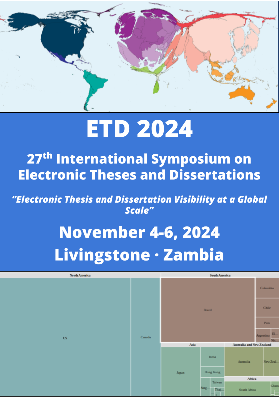
\includepdf{cover}	% our cover was produced with canva.com
	
	
% BLANK PAGE
%---------------------------------------------------------------------
\mbox{}
\thispagestyle{empty}
\vfill
\begin{center}
	\ifOnline
	The electronic version of this booklet can be found at: \\
	https://amcosconference.com/
	\else
	This is the short version of the booklet for print use. Full abstracts with all authors, references, and figures can be found in the electronic version at \url{https://amcosconference.com/}
	\fi % end if
	\\[20pt] % Please cite us by keeping the following line.
	The open-source \LaTeX{} template, AMCOS\_booklet, used to generate this booklet is available at \url{https://github.com/maximelucas/AMCOS\_booklet}
\end{center}

\newpage

% TABLE OF CONTENTS 
%---------------------------------------------------------------------
\tableofcontents

% ABOUT
%---------------------------------------------------------------------
\chapter{About}

\section{27th International Symposium on Eletronic Theses and Dissertations}
The 27th International Symposium on Electronic Theses and Dissertations (ETD 2024) aims to bring together global leaders and researchers working in the broad areas of digital libraries, institutional repositories, scholarly research and electronic theses and dissertations. The theme of ETD 2024 is "ETD Visibility at a Global Scale", and will explore innovative approaches that make use of Electronic Theses and Dissertations (ETDs), including the use of modern-day Artificial Intelligence techniques such as Large Language Models and exploration of advances that will result in increased visibility of ETDs at a Global Scale.

Thank you so very much for coming to Livingstone, Zambia to participate in the ETD 2024 conference events. We sincerely hope you enjoy the conference and your short stay in Livingstone, and, more importantly have productive and worthwhile discussions and meet new people!

Zikomo Kwambili!

\begin{minipage}[t]{\textwidth}
\raggedleft
Best Wishes\\
Lighton Phiri (Chair)
\end{minipage}

\newpage
\section{Local Conference Organizing committee}
\begin{center}
\begin{tabular}{lll}
Lighton Phiri, UNZA & Denny Nsokolo, HEA & Francina Makondo, UNZA \\
Phyela Mbewe, UNZA & Thabiso Mwiinga, UNZA &  Kaoma Daka, UNZA \\
Matildah Muchinga, LAMU  & Stein Mkandawire, ZAMREN & Buumba Dubeka, ZCAS \\
Adrian Chisale, UNZA & Dokowe Tembo, ZCAS & Cecilia Kasonde, KNU \\
Habeenzu Mulunda, UNZA & Francis Kawesha, HEA & Fabian Kakana, UNZA \\
Brian Munkondya, MU & Elijah Chileshe, UNZA & Mpande Ntumbo, ZAMREN \\
\end{tabular}

\section{Volunteers}
\begin{center}
\begin{tabular}{lll}
Mubanga Chibesa, UNZA & Gift Muwele, UNZA & Lwiimwe Shansonga, UNZA \\
Albertina Mooka, UNZA & Christabel Kunda, UNZA &  \\

\end{tabular}

\section{Programme committee}
\begin{center}
\begin{tabular}{lll}
Ana Pavani & Pontifícia Universidade Católica do Rio de Janeiro \\
Charles Greenberg & NDLTD \\
Edward Fox & Virginia Tech \\
Gabriela Mejias & DataCite \\
Hussein Suleman & University of Cape Town \\
Iryna Kuchma & EIFL \\
Jian Wu & Old Dominion University \\
Joachim Schöpfel & University of Lille \\
Lazarus Matizirofa & University of the Witwatersrand \\
Lighton Phiri & University of Zambia \\
Maïté Roux & ABES \\
Mirjana Brkovic & University of Novi Sad \\
Nabi Hasan & Indian Institute of Technology Delhi \\
Ramesh Gaur & Indira Gandhi National Centre for the Arts \\
Shantashree Sengupta & P.E.S Modern College of Arts Science and Commerce \\
Tainá Batista De Assis & Brazilian Institute of Information in Science and Technology \\
William Ingram & Virginia Polytechnic Institute and State University \\
\end{tabular}

\end{center}


% SPONSORS
%------------------------------------------------------------------
\chapter{Partner Institutions and Sponsors}

\begin{center}
The ETD 2024 conference was organised by the Networked Digital Library of Theses and Dissertations (NDLTD) and, additionally hosted by The University of Zambia (UNZA) and co-hosted by The Higher Education Authority (HEA) of Zambia and Zambia Research and Education Network (ZAMREN).
\end{center}

% % % % % \vfill

\section{Gold Sponsors}

\begin{center}

\includegraphics[width=0.20\textwidth]{images/logos/Partnerlogos/img-etd24-artwork-sponsors-proquest.png}
\end{center}

\section{Silver Sponsors}

\begin{center}

\includegraphics[width=0.15\textwidth]{images/logos/Partnerlogos/img-etd24-artwork-sponsors-ebsco.png}
\end{center}

\section{Bronze Sponsors}

\begin{center}

\includegraphics[width=0.15\textwidth]{images/logos/Partnerlogos/img-etd24-artwork-sponsors-datacite.png}

\includegraphics[width=0.15\textwidth]{images/logos/Partnerlogos/img-etd24-artwork-sponsors-uks.png}

\includegraphics[width=0.15\textwidth]{images/logos/Partnerlogos/img-etd24-artwork-sponsors-crossref.jpg}
\includegraphics[width=0.15\textwidth]{images/logos/Partnerlogos/img-etd24-artwork-sponsors-zynle.png}
\end{center}

\section{Additional Sponsors}

\begin{center}

\includegraphics[width=0.10\textwidth]{images/logos/Partnerlogos/img-etd2024-ndltd_logo.png}

\includegraphics[width=0.10\textwidth]{images/logos/Partnerlogos/img-etd2024-unza_logo.png}

\includegraphics[width=0.10\textwidth]{images/logos/Partnerlogos/img-etd2024-hea_logo.png}

\includegraphics[width=0.10\textwidth]{images/logos/Partnerlogos/img-etd2024-zamren_logo.png}

\includegraphics[width=0.10\textwidth]{images/logos/Partnerlogos/img-etd24-artwork-sponsors-datalab.png}
\end{center}

% % % % % \vfill


\newpage

% TIMETABLE 
%---------------------------------------------------------------------
\chapter{Timetable}

CT: Contributed Talk, IS: Invited Speaker, KL: Keynote Lecture, IT: Invited Talk.
% Custom commands used here can be found at the end of the preamble_booklet.tex file
\section{Day 1. Monday, November 4, 2024}

\begin{center}
% % % % % 	\filbreak
\begin{longtable}{|C{0.15\linewidth}| C{0.04\linewidth}|  C{0.3\linewidth} C{0.0\linewidth} C{0.4\linewidth}|}\hline	
% % % % % 	\tablebreak{}{Day 1. Monday, November 4, 2024}
	\tablebreak{8:30--9:00}{Registration}
	\CT{08:30--10:00}{Charles Greenberg, Hussein Suleman, Lighton Phiri}{}{NDLTD}{Workshop 1. ETDs 101: No Experience Required!}
	\CT{08:30--10:00}{Lombe Tembo}{}{ORCID}{Workshop 2. Leveraging ORCID's Global Participation Program}
	\tablebreak{10:00--10:15}{Tea/Coffee}
	\IT{10:15--10:25}{Ernest Banda}{}{Zynle Technologies Limited}{Sponsor Talk}
	\CT{10:30--13:00}{Charles Greenberg, Hussein Suleman, Lighton Phiri}{}{NDLTD}{Workshop 1. ETDs 101: No Experience Required!}
	\CT{10:15--13:00}{Lombe Tembo}{}{ORCID}{Workshop 2. Leveraging ORCID's Global Participation Program}
	\tablebreak{13:00--14:00}{Lunch}
	\CT{14:00--16:00}{Gabriela Mejias, Olatunbosun Obileye}{}{DataCite}{Workshop 3. DataCite Connect}
	\CT{14:00--16:00}{Yinlin Chen, Bill Ingram, Ed Fox}{}{Virginia Tech}{Workshop 4. Globalizing Knowledge}
	\tablebreak{16:00--16:15}{Tea/Coffee}
	\IT{16:15--16:25}{Johanssen Obanda}{}{Crossref}{Sponsor Talk}
	\CT{16:30--18:00}{Gabriela Mejias, Olatunbosun Obileye}{}{DataCite}{Workshop 3. DataCite Connect}
	\CT{16:15--18:00}{Yinlin Chen, Bill Ingram, Ed Fox}{}{Virginia Tech}{Workshop 4. Globalizing Knowledge}
	\eventtype{18:15--20:00}{NDLTD Board of Directors Meeting}
	\eventtype{18:00--20:00}{University of Zambia Ranking Committee Meeting}
\end{longtable}
\end{center}


\section{Day 2. Tuesday, November 5, 2024}

\begin{center}
% % % % % 	\filbreak
\begin{longtable}{|C{0.15\linewidth}| C{0.04\linewidth}|  C{0.3\linewidth} C{0.0\linewidth} C{0.4\linewidth}|}\hline
% % % % % 	\tablebreak{}{Day 2. Tuesday, November 5, 2024}
	\tablebreak{07:30--18:00}{Registration}
	\eventtype{08:30--09:45}{Openning Ceremony}
	\eventtype{}{Chair: Habeenzu Mulunda}
	\eventtype{}{Venue: Convention Centre}
	\tablebreak{08:30--08:35}{National Anthem}
	\tablebreak{08:35--08:40}{Prayer}
	\IS{08:40--08:50}{Lighton Phiri}{}{Chair, ETD 2024}{Welcome Remarks}
	\IS{08:50--09:00}{Edward A. Fox}{}{Executive Director, NDLTD}{Opening Remarks}
	\IS{09:00--09:10}{Stein Mkandawire}{}{CEO, Zambia Research Education Network}{Opening Remarks}
	\IS{09:10--09:20}{Trywell Kalusopa}{}{DVC of Research and Innovation, University of Zambia}{Opening Remarks}
	\IS{09:20--09:30}{Kazhila C. Chinsembu}{}{Director General, Higher Education Authority}{Opening Remarks}
	\IS{09:30--09:50}{Minister of Education}{}{Ministry of Education}{Welcome Speech}
	\KL{09:50--11:00}{Hussein Suleman}{}{University of Cape Town}{Resilience and ETD Repositories in Poor Countries}

	\eventtype{11:00--11:15}{A Moment to Remember: Official Conference Photo}

	\tablebreak{11:15--11:30}{Tea/Coffee}

	\IT{11:30--11:45}{Sylvia Kgorane}{}{ProQuest, a Part of Clarivate}{Sponsor Talk}
	\IT{11:45--11:55}{Deane Kearns}{}{EBSCO Information Services}{Sponsor Talk}

	\eventtype{12:00--13:00}{Session 1A. Infrastructure and Technologies}
	\eventtype{}{Chair: Charles Greenberg}
	\eventtype{}{Venue: Convention Centre}
	\CT{12:00--12:20}{Vivek Ranjan}{}{INFLIBNET}{Landscape of Open Access Repositories with Special Reference to Electronic Theses and Dissertations (ETD) across SAARC and BRICS Nations: A Comparative Analysis}
	\CT{12:20--12:40}{Zillur Rahman}{}{Ahsanullah University of Science and Technology}{Designing a plan for sharing ETD among the University Libraries in Bangladesh}
	\CT{12:40--12:60}{Kamani Perera}{}{Chartered Institute of Personnel Management}{Implementing Persistent Identifier Infrastructure for Effective Management of ETD Repositories: A Case Study from Chartered Institute of Personnel Management, Sri Lanka}

	\eventtype{12:00--13:00}{Session 1B. Policies and Practices}
	\eventtype{}{Chair: Gabriela Mejias}
	\eventtype{}{Venue: Convention Centre}
	\CT{12:00--12:20}{Shahzeb Hassan}{}{Akal University}{Future-Proofing Research by Long-term ETD Preservation: Challenges and Opportunities}
	\CT{12:20--12:40}{Jive Lubbungu}{}{Kwame Nkrumah University}{E-Theses and Dissertations in Zambia: A Case Study of Two Universities in Kabwe}
	\CT{12:40--12:60}{Kamani Perera}{}{Chartered Institute of Personnel Management}{Nurturing Advanced Research Culture among Medical Practitioners through ETDs: A case study from University of Kelaniya, Sri Lanka}

	\tablebreak{13:00--14:00}{Lunch}

	\eventtype{14:00--15:30}{Session 2A. Impact and Utilisation}
	\eventtype{}{Chair: Olatunbosun Obileye}
	\eventtype{}{Venue: Convention Centre}
	\CT{14:00--14:20}{Juliana Sousa}{}{Instituto Brasileiro de Informação em Ciência e Tecnologia}{Characterization of Scientific Production on Electronic Theses and Dissertations Based on a Bibliometric Analysis}
	\CT{14:20--14:40}{Mark E Phillips}{}{University Of North Texas}{Extracting and Registering References to Improve Scholarly Impact of ETDs}
	\CT{14:40--15:00}{Ana M B Pavani}{}{Pontifícia Universidade Católica do Rio de Janeiro}{International Visibility of ETDs in Portuguese and in English on a Brazilian Repository}
	\CT{15:00--15:20}{Behrooz B. Rasuli}{}{Iranian Research Institute for Information Science and Technology (IranDoc)}{Do More Complete Dissertations’ Metadata Get More Engagement?}

	\eventtype{14:00--15:30}{Session 2B. ETDs in Developing Countries}
	\eventtype{}{Chair: Hussein Suleman}
	\eventtype{}{Venue: Convention Centre}
	\CT{14:00--14:20}{Joseph P Telemala}{}{Sokoine University Of Agriculture}{Improving the Mkulima Repository Content: Utilizing Theses, Dissertations, and LLMs for Agricultural Knowledge Dissemination in Kiswahili}
	\CT{14:20--14:40}{Kenneth K Rotich}{}{Egerton University}{The Changing Landscape in Research Data Management in Kenya’s Universities: An Analysis of Development and Implementation}
	\CT{14:40--15:00}{Kamani Perera}{}{Chartered Institute Of Personnel Management}{Empowering HRM Professionals: Advancing Research Culture with ETDs in The Chartered Institute of Personnel Management (CIPM), Sri Lanka}
	\CT{15:00--15:20}{Kamani Perera}{}{Chartered Institute Of Personnel Management}{Unlocking the Potential of ETDs: Implementation Novel ETD Repository in Chartered Institute of Personnel Management in Sri Lanka}

	\tablebreak{15:30--15:45}{Tea/Coffee}

	\eventtype{15:45--17:00}{Session 3A. Infrastructure and Technologies}
	\eventtype{}{Chair: Kaoma Daka}
	\eventtype{}{Venue: Convention Centre}
	\CT{15:45--16:05}{Elijah Chileshe}{}{University of Zambia}{A Pre-Processing Pipeline for Improved ETD Metadata Quality in Downstream Services}
	\CT{16:05--16:25}{Adrian Chisale}{}{University of Zambia}{Seamless Integration of Koha and DSpace for Enhanced Management of Theses and Dissertations in Hybrid Environment: a case of University of Zambia Library}

	\eventtype{15:45--17:00}{Session 3B. ETDs in Developing Countries}
	\eventtype{}{Chair: Fabian Kakana}
	\eventtype{}{Venue: Convention Centre}
	\CT{15:45--16:05}{Mpundu Chilonga}{}{Kwame Nkruma University}{Examining the Cultural and Institutional Factors Impacting ETD Visibility in Zambia: Policy and Practice Implications}
	\CT{16:05--16:25}{Lamia Salsabil}{}{Old Dominion University}{ETD MS v2.0: A New Schema Draft for Electronic Theses and Dissertations}

	\eventtype{19:00--22:00}{Mukuni BOMA Cultural Experience Welcome Reception}
\end{longtable}
\end{center}



\section{Day 3. Wednesday, November 6, 2024}

\begin{center}
% % % % % 	\filbreak
\begin{longtable}{|C{0.15\linewidth}| C{0.04\linewidth}|  C{0.3\linewidth} C{0.0\linewidth} C{0.4\linewidth}|}\hline
% % % % % 	\tablebreak{}{Day 3. Wednesday, November 6, 2024}
	\tablebreak{07:30--18:00}{Registration}

	\eventtype{08:30--09:30}{Session 4A. Invited Talks: ETD Initiatives in Zambia}
	\eventtype{}{Chair: Denny Nsokolo}
	\eventtype{}{Venue: Convention Centre}
	\IT{08:30--08:40}{Benaia Akombwa}{}{University of Zambia}{Scholarly Research Infrastructure}
	\IT{08:45--08:55}{Zachary Zulu}{}{University of Zambia}{University of Zambia Institutional Repository}
	\IT{09:00--09:10}{Clement Sinyangwe}{}{Chalimbana University}{Chalimbana University Institutional Repository}
	\IT{09:15--09:25}{Buumba Dubeka and Dokowe Tembo}{}{ZCAS University}{ZCAS University Institutional Repository}
	\IT{09:30--09:40}{Mpundu Chilonga and Cecilia Kasonde}{}{Kwame Nkruma University}{Kwame Nkruma University Institutional Repository}
	\IT{09:45--09:55}{Eness Chitumbo and Mosebjadi Petje}{}{University of Zambia and Times Higher Education}{University Ranking}

	\eventtype{10:00--11:00}{Session 5A. Panel Discussion}
	\eventtype{}{Chair: Dokowe Tembo}
	\eventtype{}{Venue: Convention Centre}
	\IT{10:00--11:00}{How do we set up Successful ETD Projects in Zambia?}{}{Moderator: Hussein Suleman}{Participants: \hspace{5cm} Gabriela\,Mejias (DataCite) $\cdot$ Manoj\,Kumar (INFLIBNET) $\cdot$ Lighton\,Phiri (UNZA) $\cdot$ Zachary\,Zulu (UNZA)}

	\eventtype{11:00--11:30}{Session 6A. Poster/Demo Session: Minute Madness}
	\eventtype{}{Chair: Lombe Tembo}
	\eventtype{}{Venue: Convention Centre}
	\CT{11:00--11:03}{Kamani Perera}{}{Chartered Institute of Personnel Management}{Enhancing Access to Scholarly Knowledge: Strategies for Promoting Open Access ETDs in Sri Lanka}
	\CT{11:03--11:04}{Okhakhu O. David}{}{Lead City University}{Enhancing Electronic Thesis and Dissertation Visibility: A Focus on Institutional Repository Platforms and Inherent Challenges in the Nigerian Context}
	\CT{11:04--11:06}{Kamani Perera}{}{Chartered Institute of Personnel Management}{Total Quality Management in ETD Repository at Chartered Institute of Personnel Management (CIPM)}
	\CT{11:06--11:08}{Martin C Musonda}{}{University of Zambia}{Automatic Summarisation of Electronic Theses and Dissertations for Increased Media Engagement}
	\CT{11:08--11:10}{Lwiime Shansonga}{}{University of Zambia}{Automatic Electronic Thesis and Dissertation Guideline Verification For Consistently Formatted Manuscripts}
	\CT{11:10--11:12}{Elijah Chileshe}{}{University of Zambia}{Design and Implementation of an Interoperable Zambia National Electronic Thesis and Dissertation Portal}
	\CT{11:12--11:14}{Vivek Mr Ranjan}{}{INFLIBNET Center}{Exploring AI-driven strategies for enhancing the visibility of E-Theses in Shodhganga Repository}
	\CT{11:14--11:16}{Rajabu Mr Simba}{}{AHILA}{Assessing the Efficiency of Data Science Programs in Enhancing Big Data Analysis Skills among Health Libraries and Information Scientists}
	\CT{11:16--11:18}{Zainabu H LILUTU}{}{Mbeya University of Science and Technology}{Optimizing Electronic Theses and Dissertations Management for Broad Audience Engagement at Dr. Magufuli Library of Mbeya University of Science and Technology, Tanzania}
	\CT{11:18--11:20}{Zillur Rahman}{}{Ahsanullah University of Science and Technology}{Determining the factors influencing the utilization of open source digital repository software in the preservation of ETDs in academic libraries in Bangladesh}
	\CT{11:20--11:22}{Zillur Rahman}{}{Ahsanullah University of Science and Technology}{ETDs in Ensuring Quality Education for Economic Growth to Achieve Sustainable Development Goals (SDGs): Experience of SAARC Countries}
	\CT{11:22--11:24}{Mutali M Lithole}{}{University Of Johannesburg}{The University of Johannesburg’s journey to enhance the content of the Institutional Repository (IR) and improve discoverability}
	\CT{11:24--11:26}{Mduduzi Ntetha}{}{UNISA}{The conversion of printed theses and dissertations into digital formats: A case study of the University of South Africa library}
	\CT{11:26--11:28}{Sukanta  Kumar Patra}{}{Vidyasagar College for Women}{Global Visibility of National ETD Repositories of G20 Countries: comparative studies with respect to NDLTD's meta repository}
	\CT{11:28--11:30}{M A M Mominur Rahman}{}{University Of Rajshahi}{Managing ETDs in Rajshahi University Central Library : Problems and Possibilities}
	\CT{11:30--11:32}{Nobbie kandira}{}{Zimbabwe Open University}{Creating an ETD database using OMEKA. The Zimbabwe Open University Experience}

	\tablebreak{11:45--12:30}{Tea/Coffee}
	\eventtype{11:45--12:30}{Session 7A. Poster Session with Tea/Coffee}
	\eventtype{}{Chair: Thabiso Mwiinga}
	\eventtype{}{Venue: Convention Centre}

	\eventtype{12:30--13:00}{Closing Ceremony}
	\eventtype{}{Chair: Buumba Dubeka}
	\eventtype{}{Venue: Convention Centre}
	\IT{12:30--12:45}{Charles Greenberg}{}{Representative - NDLTD}{NDLTD Updates}
	\IT{12:45--13:00}{John Hagen}{}{Executive Director - USETDA}{ETD 2025 Presentation}
	\IT{12:30--12:45}{Lighton Phiri}{}{Chair - ETD 2024}{Closing Remarks}

	\tablebreak{13:00--14:00}{Lunch}

	\eventtype{14:00--15:00}{Mukuni Village Tour}
	\eventtype{14:00--15:00}{Victoria Falls Tour}
\end{longtable}
\end{center}


% TALKS 
%---------------------------------------------------------------------
\chapter{List of Abstracts -- Talks}

\section{Tuesday 20th}

% Definitions of custom environment used here can be found in preamble_booklet.tex file

% The following input commands automatically select the right version 
% (print or online) version of the abstract's .tex
% \type is defined in preamble_booklet.tex and equals:
% 'o' (online) or 'p' (print)

\input{abstracts/tex/t\type_tremblay}
\input{abstracts/tex/t\type_fournier}
\input{abstracts/tex/t\type_sato}
\input{abstracts/tex/t\type_smith}
\input{abstracts/tex/t\type_rodriguez}
\input{abstracts/tex/t\type_jansen}

\section{Thursday 22nd}

\input{abstracts/tex/t\type_schmidt}

% POSTERS
%------------------------------------------------------------------
\chapter{List of Posters} 

\vspace{-2.5em}

\section{Tuesday Session}

\input{abstracts/tex/p\type_doe}
\input{abstracts/tex/p\type_doe}
\input{abstracts/tex/p\type_doe}
\input{abstracts/tex/p\type_doe}
\input{abstracts/tex/p\type_doe}
\input{abstracts/tex/p\type_doe}
\input{abstracts/tex/p\type_doe}
\input{abstracts/tex/p\type_doe}


% LIST OF PARTICIPANTS
%------------------------------------------------------------------
\chapter{List of Participants}
 
% The array below was automatically created from a spreadsheet with 'calc2latex'

\begin{center}
\rowcolors{1}{gray!25}{white}
\begin{longtable}{p{0.25\linewidth} p{0.4\linewidth} p{0.25\linewidth}}
\hline
Austin Mclean & ProQuest, a part of Clarivate & United States \\  \hline
Bertrand Thomas & Abes & France \\  \hline
Charles Greenberg & Networked Digital Library of Theses and Dissertations & United States \\  \hline
Edward Fox & Networked Digital Library of Theses and Dissertations (NDLTD) & United States \\  \hline
Ernest Banda & Zynle Technologies Limited & Zambia \\  \hline
Gabriela Mejias & DataCite & Germany \\  \hline
Hussein Suleman & University of Cape Town & South Africa \\  \hline
Johanssen Obanda & Crossref & Kenya \\  \hline
Josiline Chigwada & University of South Africa & South Africa \\  \hline
Kudakwashe Siziva & Datacite & South Africa \\  \hline
Lamia Salsabil & Old Dominion University & United States \\  \hline
Manoj Kumar K & INFLIBNET Centre & India \\  \hline
Martin Nkumbula & Zynle Technologies Limited & Zambia \\  \hline
Mduduzi Aubrey Ntetha & University of South Africa & South Africa \\  \hline
Olatunbosun Obileye & DataCite & Nigeria \\  \hline
Olivier Cian & ABES & France \\  \hline
Shahzeb Hasan & Akal University & India \\  \hline
Vivek Ranjan & Silver Oak University & India \\  \hline
Wendel Fabian Chinsamy & DataCite & South Africa \\  \hline
\end{longtable}
\end{center}

 
% USEFUL INFO
%------------------------------------------------------------------
\chapter{Useful Information}

\textbf{Talks} will be held at the \textbf{Conference Hall-Auditorium} of PRBB. It is situated on the first floor of the central courtyard and
has independent access from the rest of the building (through stairs located at the ground floor, main entrance of PRBB). 

\textbf{Coffee breaks and lunches} will be offered in the half-covered terrace in front of the main entrance of the conference hall.

The \textbf{poster session} will be held on Tuesday and Wednesday night on the \textbf{ground floor} of the PRBB. 

Wi-Fi will be available during the conference. The PRBB also provides access to an eduroam network.

The \textbf{conference dinner} will be held at the "The best restaurant", at Some Street, 39, Barcelona.

\section{How to get to the Avani Victoria Falls Resort?}

The PRBB building overlooks the Ronda del Litoral and is next to the twin towers of the Olympic Village: Torre Mapfre and Arts Hotel. The address is Carrer del Dr. Aiguader, 88, 08003 Barcelona, Spain. and and can be reached by:

\begin{itemize}

	\item \textbf{Subway:} yellow line, L4, station Ciutadella/Vila Ol\'{i}mpica,
	\item \textbf{Bus:} lines V21, 14, 36, 41, 45, 59, 71, 92, D20,
	\item \textbf{Tram:} line 4, stop Vila Ol\'{i}mpica.
	
\end{itemize}

\subsection{Avani Victoria Falls Resort: Google Maps Location}

\begin{center}
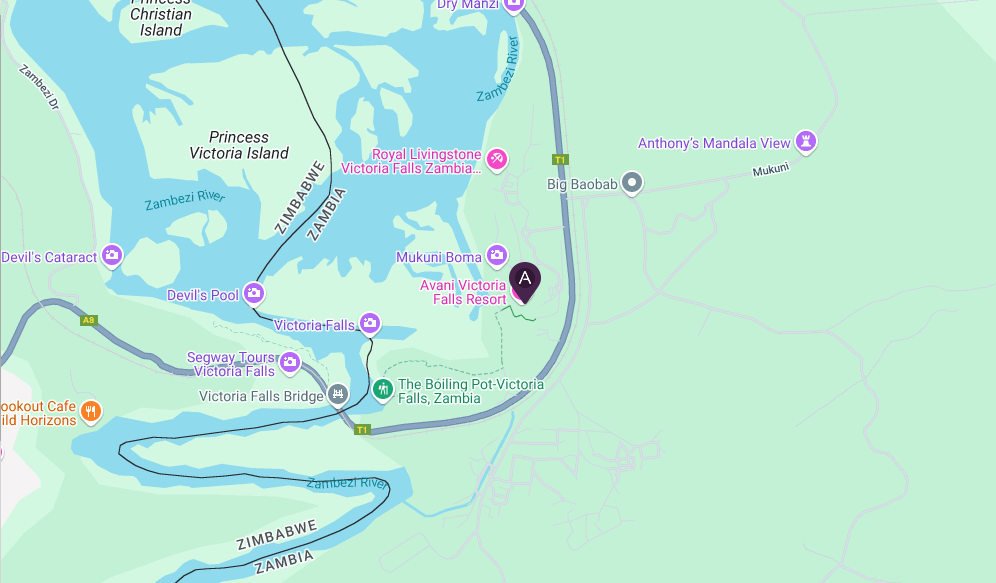
\includegraphics[width=\linewidth]{images/img-etd24-avani_victoria_fall_convention_centre_map.png}
\end{center}


\subsection{Avani Victoria Falls Resort: Convention Centre Layout}

\begin{center}
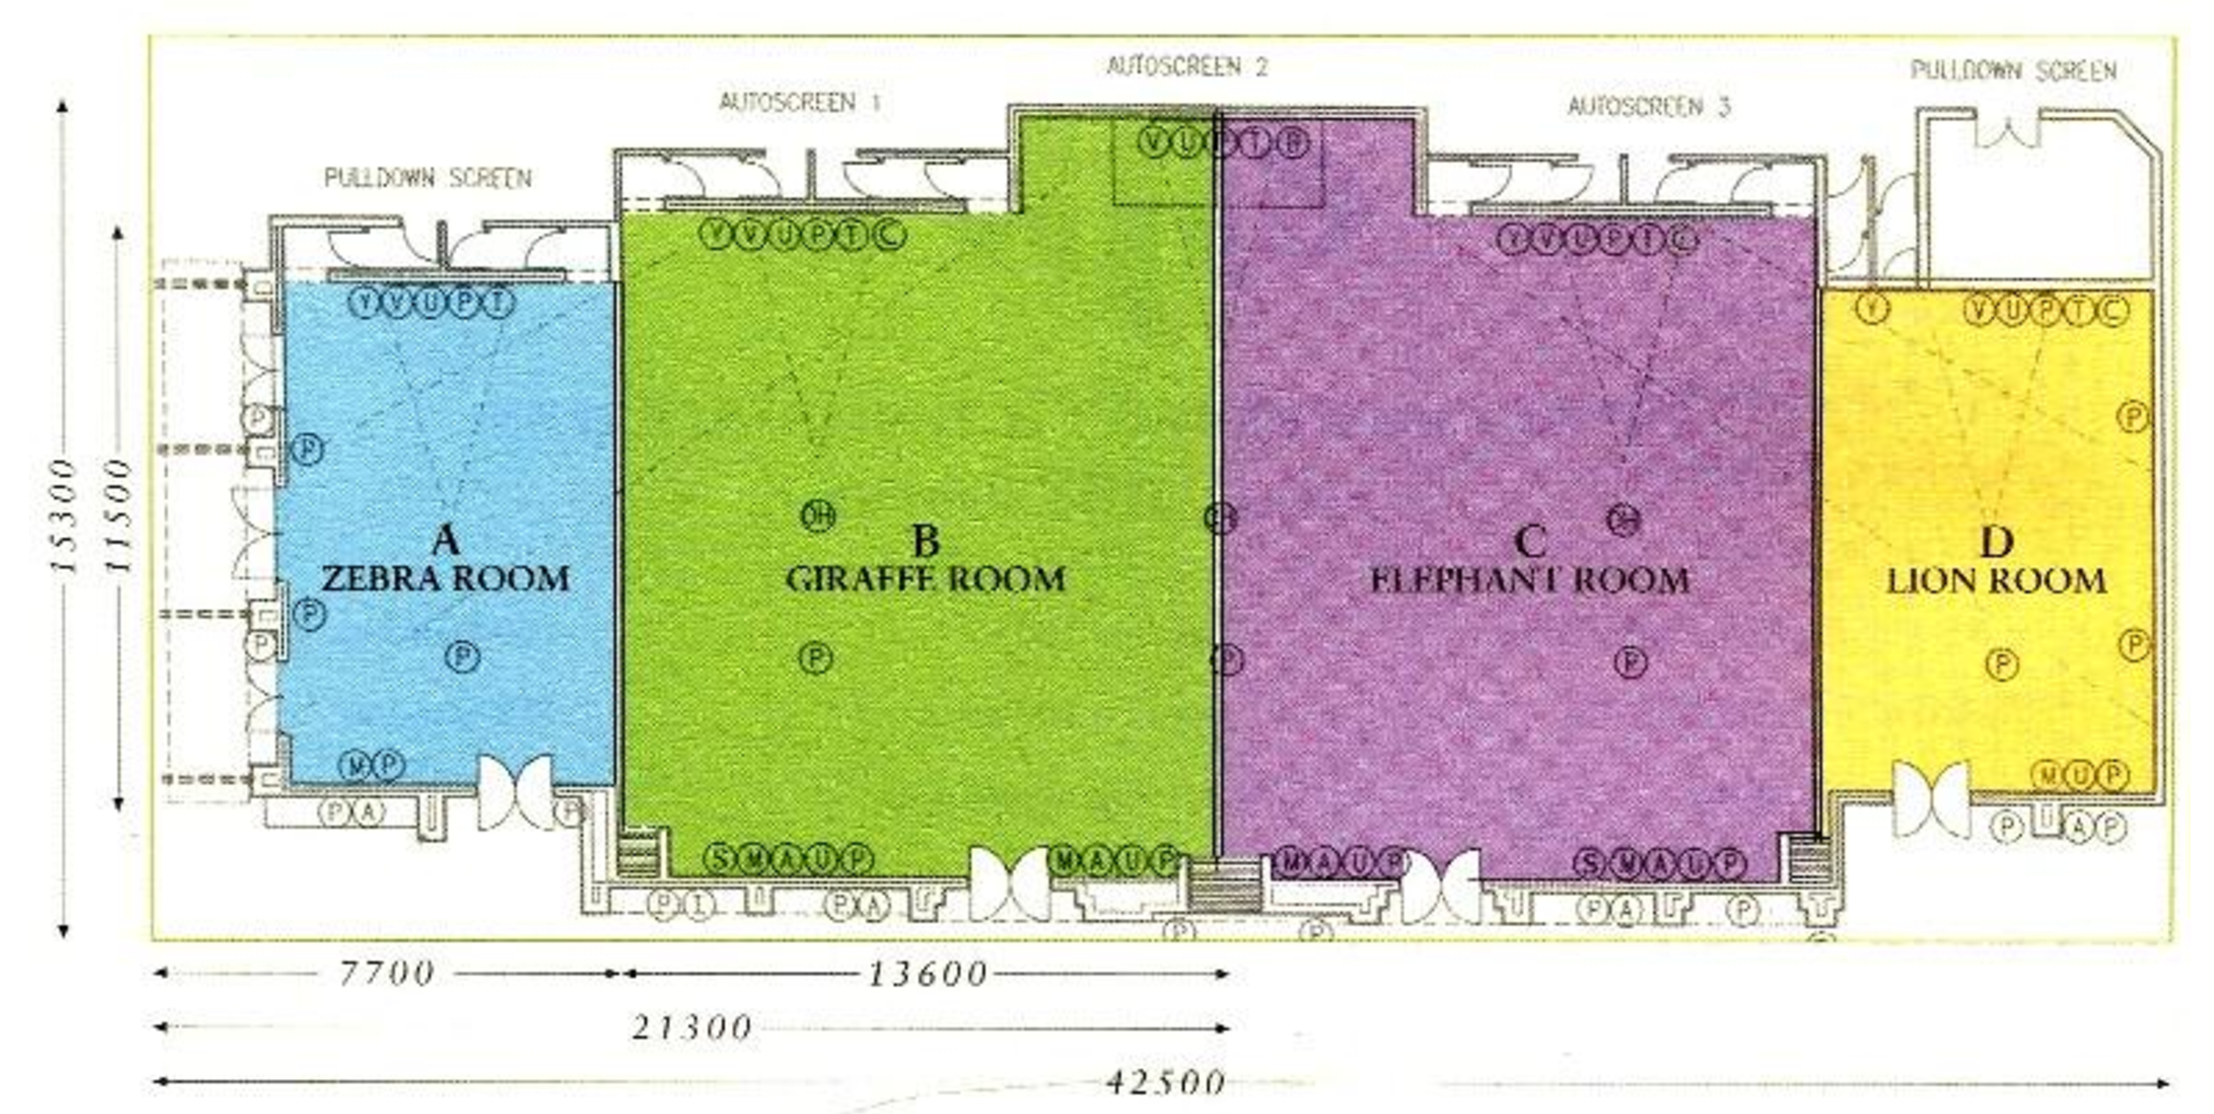
\includegraphics[width=\linewidth]{images/img-etd24-avani_victoria_fall_convention_centre_layout.png}
\end{center}


% % % % % % SPONSORS
% % % % % %------------------------------------------------------------------
% % % % % \chapter{Partner Institutions and Sponsors}
% % % % %
% % % % % \begin{center}
The ETD 2024 conference was organised by the Networked Digital Library of Theses and Dissertations (NDLTD) and, additionally hosted by The University of Zambia (UNZA) and co-hosted by The Higher Education Authority (HEA) of Zambia and Zambia Research and Education Network (ZAMREN).
\end{center}

% % % % % \vfill

\section{Gold Sponsors}

\begin{center}

\includegraphics[width=0.20\textwidth]{images/logos/Partnerlogos/img-etd24-artwork-sponsors-proquest.png}
\end{center}

\section{Silver Sponsors}

\begin{center}

\includegraphics[width=0.15\textwidth]{images/logos/Partnerlogos/img-etd24-artwork-sponsors-ebsco.png}
\end{center}

\section{Bronze Sponsors}

\begin{center}

\includegraphics[width=0.15\textwidth]{images/logos/Partnerlogos/img-etd24-artwork-sponsors-datacite.png}

\includegraphics[width=0.15\textwidth]{images/logos/Partnerlogos/img-etd24-artwork-sponsors-uks.png}

\includegraphics[width=0.15\textwidth]{images/logos/Partnerlogos/img-etd24-artwork-sponsors-crossref.jpg}
\includegraphics[width=0.15\textwidth]{images/logos/Partnerlogos/img-etd24-artwork-sponsors-zynle.png}
\end{center}

\section{Additional Sponsors}

\begin{center}

\includegraphics[width=0.10\textwidth]{images/logos/Partnerlogos/img-etd2024-ndltd_logo.png}

\includegraphics[width=0.10\textwidth]{images/logos/Partnerlogos/img-etd2024-unza_logo.png}

\includegraphics[width=0.10\textwidth]{images/logos/Partnerlogos/img-etd2024-hea_logo.png}

\includegraphics[width=0.10\textwidth]{images/logos/Partnerlogos/img-etd2024-zamren_logo.png}

\includegraphics[width=0.10\textwidth]{images/logos/Partnerlogos/img-etd24-artwork-sponsors-datalab.png}
\end{center}

% % % % % \vfill

% % % % %
% % % % % \newpage

% BACK PAGE
%-----------------------------------------------------------------

\pagecolor{myblue}
\thispagestyle{empty}
\mbox{}

\end{document}
